%%%%%%%%%%%%%%%%%%%%%%%%% PAGESETUP %%%%%%%%%%%%%%%%%%%%%%%%%
% Document class
\documentclass[12pt,a4paper]{report}
% Alternative Options:
%	Paper Size: a4paper / a5paper / b5paper / letterpaper / legalpaper / executivepaper
% Duplex: oneside / twoside
% Base Font Size: 10pt / 11pt / 12pt
%%%%%%%%%%%%%%%%%%%%%%%%% Packages %%%%%%%%%%%%%%%%%%%%%%%%%%
\usepackage[utf8]{inputenc} % Bruges til at gengive bogstaver
\usepackage{array} % Bruges til tabeller
\usepackage{natbib} % Bruges til referencer
\usepackage{graphicx} % Bruges til at indsætte billeder
\graphicspath{{Images/}} %Specifies that all images are placed in the Images folder
\usepackage{fancyhdr} % Bruges til headers og footers
\usepackage{lastpage} % Bruges til at finde sidste sidetal
\usepackage[danish]{babel} % Ændre standardfraser til dansk
\usepackage{hyperref} % Bruges til at tilføje hyperlinks, also allows the use of \autoref{}
\hypersetup{linktoc=all} 

\usepackage[all]{hypcap} % Bruges til at linke til toppen af en figur
\usepackage{pdfpages} % Bruges til at indlæse pdfer
\usepackage{amsmath, amssymb, amsthm} % Math-stuffs
\usepackage[a4paper, headheight=27.06pt]{geometry} % Sætter marginer i dokumentet
\usepackage{microtype} % Gør teksten mere læsevenlig
\usepackage{siunitx} % tillader at bruge \SI{10}{\hertz}
\sisetup{per-mode=fraction,
		 exponent-product=\cdot,
		 range-units=single,
		 range-phrase=\ til\ }
		 
\usepackage[parfill]{parskip} % Removes the indentation at new paragraphs
\usepackage{mcode} % Used to input matlab figures, requires matlab code as well
\lstset{inputencoding=utf8}

\usepackage{float} % Allows the terrible use of [H] as a float identifier
%%%%%%%%%%%%%%%%%%%%%%% END PAGESETUP %%%%%%%%%%%%%%%%%%%%%%%

%Double underline for use in math problems
\newcommand{\facit}[1]{\underline{\underline{#1}}}

%Project specific commands
\newcommand{\GFS}{\SI{44.1}{\kilo\hertz} }
\newcommand{\GFN}{\SI{22.05}{\kilo\hertz} }
\newcommand{\FS}{\SI{22.05}{\kilo\hertz} }
\newcommand{\FN}{\SI{11.025}{\kilo\hertz} }
\newcommand{\degree}{^{\circ}}

%Approved/Dissaproved symbols
\newcommand{\OK}{$\textcolor{green}{\checkmark}$}
\newcommand{\NO}{$\textcolor{red}{\times}$}

%Allows the use of * as \cdot in math
\mathcode`\*="8000
{\catcode`\*\active\gdef*{\cdot}}
%%%%%%%%%%%%%%%%%%%%%%%%%%%%%%%%%%%%%%%%%%%%%%%%%%%%%%%%%%%%%
%%%%%%%%%%%%%%%%%%%%%%%%%% AUTHORS %%%%%%%%%%%%%%%%%%%%%%%%%%
% Elev A
\newcommand{\StudentNumberA}{Sxxxxxx}
\newcommand{\StudentNameA}{Student 1}
\newcommand{\StudentPictureA}{Forsider/Profile.png} 
% Elev B
\newcommand{\StudentNumberB}{Sxxxxxx}
\newcommand{\StudentNameB}{Student 2}
\newcommand{\StudentPictureB}{Forsider/Profile.png}
% Elev C
\newcommand{\StudentNumberC}{Sxxxxxx}
\newcommand{\StudentNameC}{Student 3}
\newcommand{\StudentPictureC}{Forsider/Profile.png}
% Elev D
\newcommand{\StudentNumberD}{Sxxxxxx}
\newcommand{\StudentNameD}{Student 4}
\newcommand{\StudentPictureD}{Forsider/Profile.png}
%%%%%%%%%%%%%%%%%%%%%%%% END AUTHORS %%%%%%%%%%%%%%%%%%%%%%%%
%%%%%%%%%%%%%%%%%%%%%%%%%%%%%%%%%%%%%%%%%%%%%%%%%%%%%%%%%%%%%
%%%%%%%%%%%%%%%%%%%%%%%% COURSE INFO %%%%%%%%%%%%%%%%%%%%%%%%
\newcommand{\Course}{Digital Signalbehandling} %Indsæt klassenavn
\newcommand{\CourseNumber}{62738} %Indsæt klassenummer
\newcommand{\ProjectName}{Kursusopgave 5} %Indsæt projektnavn
\newcommand{\GroupNumber}{} %Gruppenummer

%%%%%%%%%%%%%%%%%%%%% INSERT FRONT PAGE %%%%%%%%%%%%%%%%%%%%%
\begin{document}


%%%%%%%%%%%%%%%%%%%%%%%%%%%%%%%% FRONTPAGE %%%%%%%%%%%%%%%%%%%%%%%%%%%%%%%
\begin{titlepage}
	\centering
	
\includegraphics[scale=0.3]{Forsider/DTUlogo.png}\par
	\vspace{0.5cm}
	{\LARGE \CourseNumber \par}
	{\LARGE \Course \par}
	\vspace{1.5cm}
	{\textbf{\Huge \ProjectName}\par} %
	{\today\par} %Dato
	\vspace{3cm}
	\begin{tabular}{>{\centering}m{4cm}|>{\centering}m{4cm}|>{\centering}m{4cm}}
    \textbf{\large{\StudentNumberA}} & 
    \textbf{\large{\StudentNumberB}} & 
    \textbf{\large{\StudentNumberD}}                            \tabularnewline
    
    \includegraphics[scale=0.7]{\StudentPictureA}\par &
    \includegraphics[scale=0.7]{\StudentPictureB}\par &
    \includegraphics[scale=0.7]{\StudentPictureD}\par           \tabularnewline
    
    \textbf{\StudentNameA} & 
    \textbf{\StudentNameB} & 
    \textbf{\StudentNameD}                                      \tabularnewline
    
    
    \end{tabular}\par
    \end{titlepage}
%%%%%%%%%%%%%%%%%%%%%%%%%%%%%% END FRONTPAGE %%%%%%%%%%%%%%%%%%%%%%%%%%%%%%
%%%%%%%%%%%%%%%%%%% END INSERT FRONT PAGE %%%%%%%%%%%%%%%%%%%
%%%%%%%%%%%%%%%%%%%%%%%%%%%%%%%%%%%%%%%%%%%%%%%%%%%%%%%%%%%%%
%%%%%%%%%%%%%%%%%%%% HEADERS AND FOOTERS %%%%%%%%%%%%%%%%%%%%
\pagestyle{fancy}
\fancyhf{}
\chead{DTU\\  \CourseNumber\ - \Course}
\rhead{Chapter \thechapter}
\lhead{\GroupNumber}
\rfoot{Page \thepage/\pageref*{LastPage}}
%%%%%%%%%%%%%%%%%% END HEADERS AND FOOTERS %%%%%%%%%%%%%%%%%%
%%%%%%%%%%%%%%%%%%%%%%%%%%%%%%%%%%%%%%%%%%%%%%%%%%%%%%%%%%%%%
%%%%%%%%%%%%%%%%%%%%% TABLE OF CONTENTS %%%%%%%%%%%%%%%%%%%%%
\tableofcontents
\thispagestyle{fancy}
\newpage
%%%%%%%%%%%%%%%%%%% END TABLE OF CONTENTS %%%%%%%%%%%%%%%%%%%
%%%%%%%%%%%%%%%%%%%%%%%%%%%%%%%%%%%%%%%%%%%%%%%%%%%%%%%%%%%%%
%%%%%%%%%%%%%%%%%%%%%%% ACTUAL REPORT %%%%%%%%%%%%%%%%%%%%%%%



%Section/Chapter without numbering on the page, but still added to the ToC
\section*{Forord}
\addcontentsline{toc}{chapter}{\protect\numberline{}Forord}%
The part that goes in the section
%END




%Chapter without numbering on page, but still added to ToC
\chapter*{ChapterName}
\setcounter{chapter}{1}
\setcounter{section}{0}
\addcontentsline{toc}{chapter}{\protect\numberline{}ChapterName}
\thispagestyle{fancy} %Using fancyheader
\label{ch:ChapterReference}
%%%%%%%%%%%%%%%%%%%%%%%%%%%%%%%%%%%%%%%%%%

%Bullet list
\begin{itemize}
    \item sampling frekvens: $f_s$ = \FS 
    \item 3 dB båndbredde: BW = 25 Hz
    \item Center frekvens: $f_0$ = 50 Hz
\end{itemize}
%%%%%%%%%%%%%%%%%%%%%%%%%%%%%%%%%%%%%%%%%%

%Equation
\begin{equation}
    r = 1 -\bigg(\frac{BW_{3dB}}{f_s}\bigg)\cdot\pi \implies
    1-\bigg(\frac{\SI{25}{\hertz}}{\FS}\bigg)\cdot\pi = 0.9964381036
\end{equation}
%%%%%%%%%%%%%%%%%%%%%%%%%%%%%%%%%%%%%%%%%%

%Insert image
\begin{figure}[H]%[H] requires the float package, standard options are [htb!]
\center
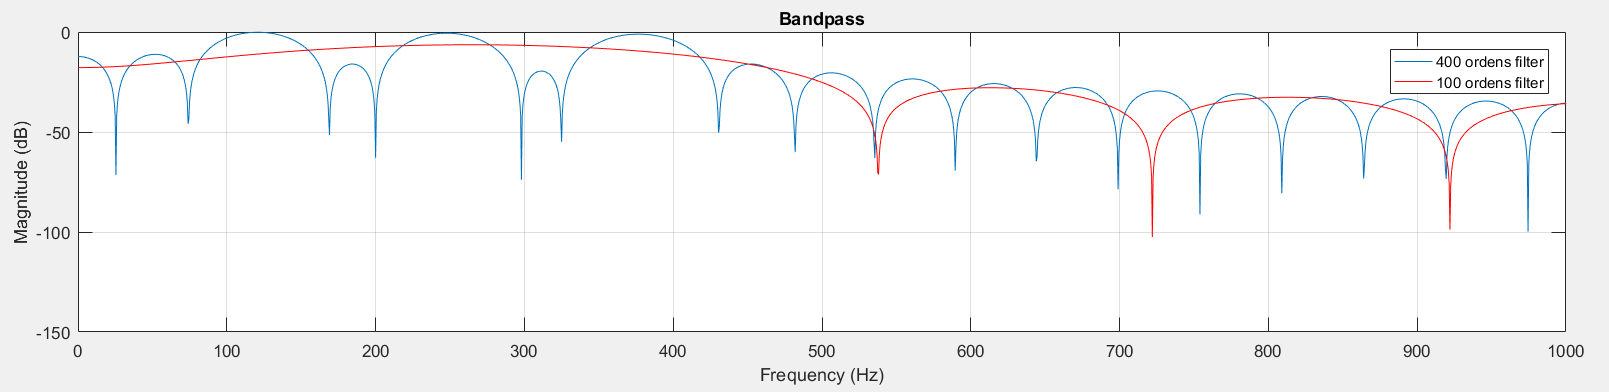
\includegraphics[scale=0.7]{NameOfImage}
\caption{Caption text goes here}
\label{fig:Reference}
\end{figure}
%%%%%%%%%%%%%%%%%%%%%%%%%%%%%%%%%%%%%%%%%%

%Aligned equations
\begin{align}
   f_h = f_0 + \frac{W_{pass}}{2} &\implies \SI{50}{\hertz} + \frac{\SI{50}{\hertz}}{2} = \SI{75}{\hertz}\\
   f_l = f_0 + \frac{W_{pass}}{2} &\implies \SI{50}{\hertz} - \frac{\SI{50}{\hertz}}{2} = \SI{25}{\hertz}\\
   T=\frac{1}{f_s} &\implies \frac{1}{\FS}
\end{align}
%%%%%%%%%%%%%%%%%%%%%%%%%%%%%%%%%%%%%%%%%%

\begin{equation}
\begin{aligned}
  &\omega_{ah} = \frac{2}{T}*tan\bigg(\frac{\omega_h*T}{2}\bigg) \implies\\ &44100*tan\bigg(\frac{150*\pi/\FS}{2}\bigg) = \SI{471.2568349}{\radian\per\second}
  \end{aligned}
\end{equation}

%Math in text
Der vælges $\omega_{ah}=\SI{471.2568349}{\radian\per\second},\ \omega_{al}=\SI{209.4386244}{\radian\per\second},\ \omega_{sh}=\SI{392.7094616}{\radian\per\second}$ og $\omega_{sl}=\SI{251.3292724}{\radian\per\second}$ for at få den smalleste bredde, så der fjernes så lidt muligt af frekvenserne tæt ved 50 Hz.
%%%%%%%%%%%%%%%%%%%%%%%%%%%%%%%%%%%%%%%%%%

%Table in figure
\begin{figure}[H]
\centering
\begin{tabular}{c c}
  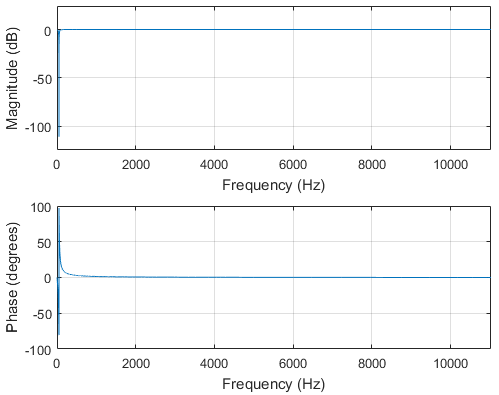
\includegraphics[scale=0.52]{Freqz_P-Z}  & 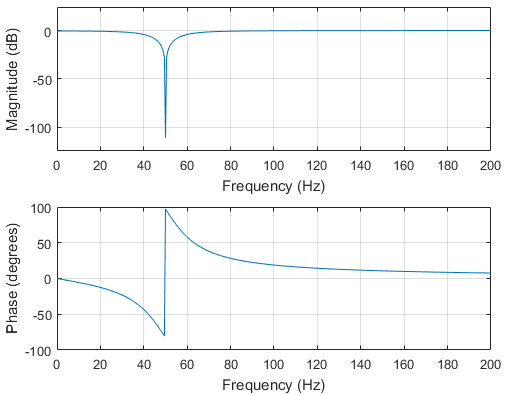
\includegraphics[scale=0.52]{Freqz_P-Z_zoom} 
\end{tabular}
\caption{Caption text here}
\label{tab:Reference}
\end{figure}
%%%%%%%%%%%%%%%%%%%%%%%%%%%%%%%%%%%%%%%%%%

%Labeled section
\section{Design}
\subsection{Frekvenser i et D}\label{subsec:FrekD}
%%%%%%%%%%%%%%%%%%%%%%%%%%%%%%%%%%%%%%%%%%

%Image from Matlab, using M-code to Latex
\begin{figure}[H]
    \centering
    \scalebox{0.45}{
    \input{Figurer/Blackman.pdf_tex}}
    \caption{Plot af et Blackmanvindue med 1201 samples}
    \label{fig:Blackman}
\end{figure}
%%%%%%%%%%%%%%%%%%%%%%%%%%%%%%%%%%%%%%%%%%

%Enumaration
Metode:
\begin{enumerate}
    \item Først bestemmes amplituden ved hver af fr diskrete frekvenser mellem 0 og Nyquist. Disse frekvenser findes ved følgende formel:
    \begin{equation}
       H_k \ @ \  \Omega_k = \frac{2\pi k}{2M+1},\ \ k = 0, 1, ..., M
    \end{equation}
    \item Herefter invers fourier transformeres disse ved brug af følgende forsimplede regneudtryk, som antager lineær fase:
    \begin{equation}
        b_n \ = \ h(n) \ = \ \frac{1}{2M+1}\bigg(H_0 + 2\sum\limits_{k=1}^M H_k \ cos\bigg(\frac{2\pi k(n-M)}{2M+1}\bigg)\bigg)
    \end{equation}
    \item Til sidst findes resten af filterkoeficienterne, som, grundet antagelsen om lineær fase, er magen til de beregnede, men spejlvendt (den sidste koefficient spejles dog ikke).
    \begin{equation}
        h(n) \ = h(2M-n), \ \ n=M+1,...,2M
    \end{equation}
\end{enumerate}
%%%%%%%%%%%%%%%%%%%%%%%%%%%%%%%%%%%%%%%%%%

%Table
\begin{center}
\begin{tabular}{| c | c | c |}
\hline
$F_s$ & Sampling frekvens & \SI{22.05}{\kilo\hertz}\tabularnewline
\hline
$F_c$ & Center frekvens & \SI{150}{\hertz}\tabularnewline
\hline
$BW$ & Båndbredde & \SI{50}{\hertz}\tabularnewline
\hline
\end{tabular}
\end{center}

%Using fixed cell sizes
\begin{center}
\begin{tabular}{||m{1cm}|m{1cm}|m{1cm}||}
\hline
    jasd & joke & lol\tabularnewline
    \multicolumn{3}{c}{Samlet tekst}\tabularnewline
    sokd & dsofksdof & sodfosd\tabularnewline
\hline
\end{tabular}
\end{center}
%%%%%%%%%%%%%%%%%%%%%%%%%%%%%%%%%%%%%%%%%%

%Code input using lstlisting package
%Part of a file
\lstinputlisting[firstline=1, lastline=3]{Matlab/kursus_opg_5_mads.m}

\lstinputlisting[firstline=20, lastline=30]{Matlab/kursus_opg_5_mads.m}

%Or entire file
\lstinputlisting{Matlab/Opg5_bandstop.m}
%%%%%%%%%%%%%%%%%%%%%%%%%%%%%%%%%%%%%%%%%%




\chapter*{Konklusion}
\setcounter{chapter}{9}
\setcounter{section}{0}
\addcontentsline{toc}{chapter}{\protect\numberline{}Konklusion}%
\thispagestyle{fancy}
%%%%%%%%%%%%%%%%%%%%%%%%%%%%%%%%%%%%%%%%%%
Ud fra delkonklusionerne vurderes det, at filtrene der er lavet, fungere efter hensigten. Samtidigt fungere systemet til dels som ønsket, da ord indeholdende "d" eller "e" bliver fremhævet fra talestrømmen. Det vurderes dog, at det ikke passende måde, at implementere stemmegenkendelse, da der forefindes stor varians i frekvensindholdet af ord, alt efter udtale, stemmeleje, mm. 


\end{document}
